\documentclass{beamer}
%\usepackage[margin=1in]{geometry}
\usepackage{amsthm,amsmath,amsfonts,hyperref,graphicx,color,multicol}
\usepackage{enumitem,tikz}
\usepackage{booktabs}
%%%%%%%%%%
%Beamer Template Customization
%%%%%%%%%%
\setbeamertemplate{navigation symbols}{}
\setbeamertemplate{theorems}[ams style]
\setbeamertemplate{blocks}[rounded]

\definecolor{Blu}{RGB}{43,62,133} % UWEC Blue
\setbeamercolor{structure}{fg=Blu} % Titles

%Unnumbered footnotes:
\newcommand{\blfootnote}[1]{%
	\begingroup
	\renewcommand\thefootnote{}\footnote{#1}%
	\addtocounter{footnote}{-1}%
	\endgroup
}


%%%%%%%%%%
%Custom Commands
%%%%%%%%%%
\newcommand{\R}{\mathbb{R}}
\newcommand{\veca}{\vec{a}}
\newcommand{\vecb}{\vec{b}}
\newcommand{\vece}{\vec{e}}
\newcommand{\vecu}{\vec{u}}
\newcommand{\vecv}{\vec{v}}
\newcommand{\vecw}{\vec{w}}
\newcommand{\vecx}{\vec{x}}
\newcommand{\zerovector}{\vec{0}}

\newcommand{\ds}{\displaystyle}

\newcommand{\fn}{\insertframenumber}

\newcommand{\col}{\operatorname{col}}
\newcommand{\row}{\operatorname{row}}
\newcommand{\rank}{\operatorname{rank}}
\newcommand{\nullity}{\operatorname{nullity}}
\newcommand{\adj}{\operatorname{adj}}
\newcommand{\proj}{\operatorname{proj}}
\newcommand{\ip}[2]{\left\langle #1,#2\right\rangle}

\newcommand{\blank}[1]{\underline{\hspace*{#1}}}

\newcommand{\dotp}{\,{\boldsymbol{\cdot}\hspace*{.01in}}}

%%%%%%%%%%
%Custom Theorem Environments
%%%%%%%%%%
\theoremstyle{definition}
\newtheorem{exercise}{Exercise}
\newtheorem{question}[exercise]{Question}
\newtheorem*{defn}{Definition}
\newtheorem*{exa}{Example}
\newtheorem*{disc}{Group Discussion}
\newtheorem*{nb}{Note}
\newtheorem*{recall}{Recall}
\renewcommand{\emph}[1]{{\color{blue}\texttt{#1}}}

\definecolor{Gold}{RGB}{237, 172, 26}
%Statement block
\newenvironment{statementblock}[1]{%
	\setbeamercolor{block body}{bg=Gold!20}
	\setbeamercolor{block title}{bg=Gold}
	\begin{block}{\textbf{#1.}}}{\end{block}}





\begin{document}
	\title{Math 324: Linear Algebra}
	\subtitle{Section 6.1: Linear Transformations}
	\author{Mckenzie West}
	\date{Last Updated: \today}
\begin{frame}
\maketitle
\end{frame}

\begin{frame}{\insertframenumber}
	\begin{block}{\textbf{Last Time.}}
	\begin{itemize}[label=--]
		\item Exam 2: Vector Spaces, Matrix Spaces, Inner Products
	\end{itemize}
	\end{block}
	\begin{block}{\textbf{Today.}}
		\begin{itemize}[label=--]
			\item Linear Transformations
			\item Properties of Linear Transformations
			\item Matrix Transformations
		\end{itemize}
	\end{block}
\end{frame}
\begin{frame}{\fn}
	\begin{defn}
		A \emph{transformation} from $V$ to $W$, a.k.a.\ \emph{function} or \emph{mapping}, denoted by $T\colon V\to W$ is a pairing that assigns to each element in the \emph{domain} $V$ exactly one element in the \emph{codomain} $W$.
	\end{defn}
	\begin{exa}
		In Calculus I and II, we use functions whose domains are subsets of $\R$ and codomains are $\R$, such as 
			\begin{itemize}[label=--]
				\item $f\colon\R\to\R$ defined by $f(x)=x^2$
				\item or $g\colon[-1,1]\to\R$ defined by $g(x)=\sqrt{1-x^2}$.
			\end{itemize}
	\end{exa}
	\begin{nb}
		Notice that the codomain is different from the \emph{range} which is the elements in the codomain that are \textit{hit} by the map.
	\end{nb}
\end{frame}
\begin{frame}{\fn}
	\begin{exercise}
		Consider the mapping $T:\R^2\to P_1$ defined by $$T((a,b))=(a^2+b^2x).$$
			\begin{enumerate}[label=(\alph*)]
				\item Compute $T((3,-2))$.
				\item What is the domain of $T$?
				\item What is the codomain of $T$?
				\item What is the range of $T$?
			\end{enumerate}
	\end{exercise}
\end{frame}
\begin{frame}{\fn}
	\begin{defn}
		If $T:V\to W$ is a transformation, the \emph{image} of $\vec v$ under $T$ is the value $T(\vec v)$ in $W$ that has been assigned to $\vec v$.
		
		For $\vec w\in W$, the \emph{preimage} of $\vec w$, denoted $T^{-1}(\vec w)$, is the collection of \textit{all} vectors $\vec v$ in $V$ for which $T(\vec v)=\vec w$.  
		In set notation, \[T^{-1}(\vec w)=\{\vec v\in V : T(\vec v)=\vec w\}.\]
	\end{defn}
	\begin{exercise}
	Again using the mapping $T:\R^2\to P_1$ defined by $$T((a,b))=(a^2+b^2x).$$
		\begin{enumerate}[label=(\alph*)]
			\item What is the image of $(-2,2)$?
			\item What is the preimage of $1+x$?
			\item What is the preimage of $-2x$?
		\end{enumerate}
	\end{exercise}
\end{frame}
\begin{frame}{\fn}
	\begin{defn}
		If $V$ and $W$ are vector spaces, a \emph{linear transformation} from $V$ to $W$ is a mapping $T\colon V\to W$ that satisfies
			\begin{enumerate}[label=\textbf{\arabic*.}]
				\item $T(\vec v_1+\vec v_2)=T(\vec v_1)+T(\vec v_2)$ for all $\vec v_1,\vec v_2\in V$,
				\item and $T(c\vec v)=cT(\vec v)$ for all scalars $c$ and $\vec v\in V$.
			\end{enumerate}
	\end{defn}
	\begin{exa}
		The mapping $T:\R^2\to\R^2$ given by $T(\vec v)=2\vec v$ is a linear transformation because
		\begin{enumerate}[label=\textbf{\arabic*.}]
			\item $T(\vec v_1+\vec v_2)=2(\vec v_1+\vec v_2)=2\vec v_1+2\vec v_2=T(\vec v_1)+T(\vec v_2)$
			\item $T(c\vec v)=2(c\vec v)=c(2\vec v)=cT(\vec v)$
		\end{enumerate}
	\end{exa}
\end{frame}
\begin{frame}{\fn}
	\begin{exercise}
		Which of the following functions are linear transformations?
		\begin{enumerate}[label=(\alph*)]
			\item $T:\R^2\to\R^3$, $T(x,y)=(2y-x,x,y)$
			\item $T:\R^2\to P_1$, $T(a,b)=a^2+b^2x$
			\item $T:M_{2,2}\to \R$, $T(A)=\det(A)$
			\item $T:\R^3\to M_{2,2}$, $T(x,y,z)=\begin{bmatrix}x&y\\z&x+y+z\end{bmatrix}$
		\end{enumerate}
	\end{exercise}
\end{frame}
\begin{frame}{\fn}
	\begin{exa}
		Here are some important linear transformations, you may want to make sure you believe they are linear transformations.
		\begin{enumerate}[label=(\alph*)]
			\item $T:M_{m,n}\to M_{n,m}$, $T(A)=A^T$
			\item $D:P_n\to P_{n-1}$, $D(p)=p'$\\
			 (works when the domain and codomain are the collection of all differentiable functions too)
			\item $I:P_n\to \R$, $\ds I(p)=\int_a^b p(x)\ dx$
		\end{enumerate}
	\end{exa}
\end{frame}
\begin{frame}{\fn}
	\begin{statementblock}{Theorem 6.1}
		Let $T\colon V\to W$ be a linear transformation and $\vec u$, $\vec v\in V$.  Then the following are true
			\begin{enumerate}[label=\textbf{\arabic*.}]
				\item $T(\vec 0_V)=\vec 0_W$
				\item $T(-\vec v)=-T(\vec v)$
				\item $T(\vec u-\vec v)=T(\vec u)-T(\vec v)$
				\item $T(c_1\vec v_1+c_2\vec v_2+\cdots+c_n\vec v_n)=c_1T(\vec v_1)+c_2T(\vec v_2)+\cdots+c_nT(\vec v_n)$
			\end{enumerate}
	\end{statementblock}
	\begin{exercise}
		Prove properties 1 and 2, being sure to reference Theorem 4.4, which states $0\vec v=\vec 0$ and $-\vec v=(-1)\vec v$.
	\end{exercise}
\end{frame}
\begin{frame}{\fn}
	\begin{nb}
		The last property of Theorem 6.1 indicates the strength of linear transformations.
		
		In particular if $S=\{\vec v_1,\vec v_2,\dots,\vec v_n\}$ is a basis for the vector space $V$, then any linear transformation $T\colon V\to W$ can be described solely by $T(\vec v_1)$, $T(\vec v_2)$, \dots, $T(\vec v_n)$, as in the video
		\begin{center}
			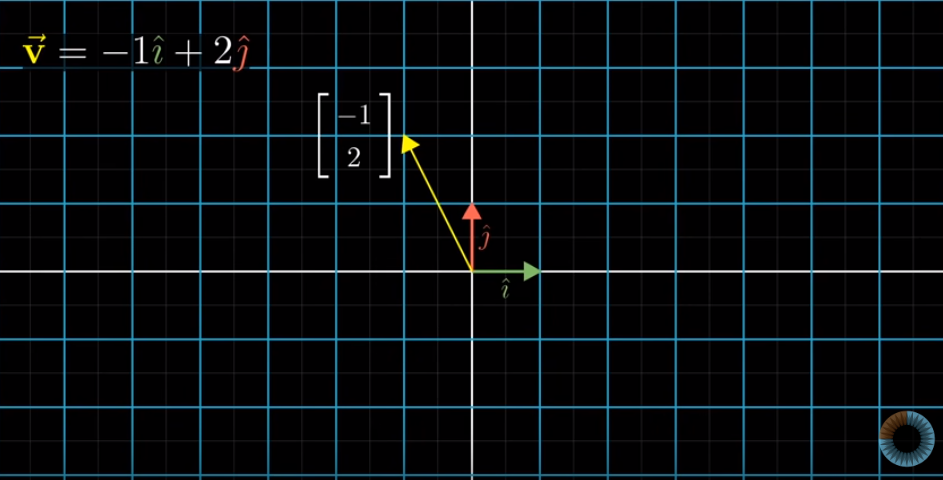
\includegraphics[width=.4\textwidth]{images/linear_transformation_basis_1}
			\hspace{.25in}
			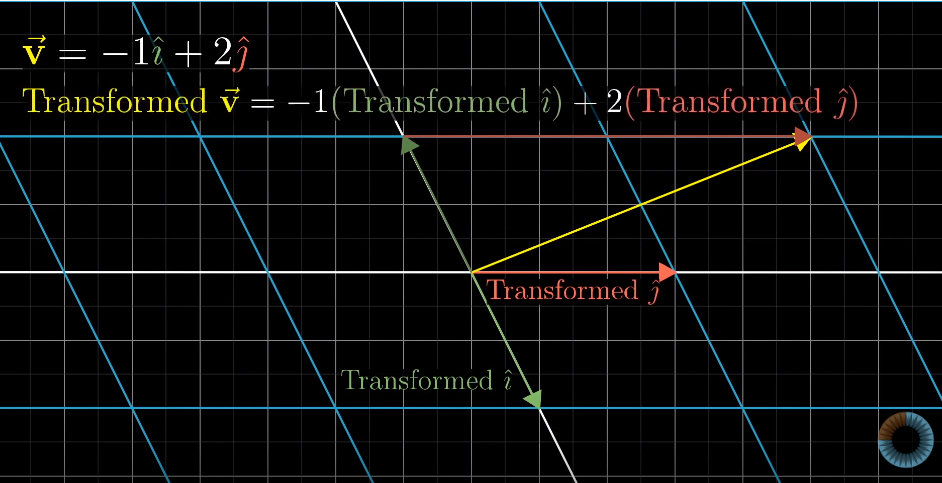
\includegraphics[width=.4\textwidth]{images/linear_transformation_basis_2}
		\end{center}
	\end{nb}
\end{frame}
\begin{frame}{\fn}
	\begin{exercise}
		Let $T:\R^3\to \R^2$ satisfy $T(1,0,0)=(1,1)$, $T(0,1,0)=(2,1)$, and $T(0,0,1)=(0,-3)$.
		\begin{enumerate}[label=(\alph*)]
			\item What is $T(1,2,3)$?
			\item What is $T(x,y,z)$?
		\end{enumerate}
	\end{exercise}
\end{frame}
\begin{frame}{\fn}
	\begin{block}{\textbf{Brain Break.}}
		What is your favorite fruit?
		\begin{center}
			
\includegraphics[height=.3\textheight]{images/fruit}
		\end{center}
	
		My favorite fruit is probably a raspberry.
	\end{block}
\end{frame}
\begin{frame}{\fn}
	\begin{exercise}
		Let $T:\R^2\to \R^4$ satisfy $T(1,2)=(1,2,0,0)$ and $T(2,1)=(0,0,2,1)$. 
		\begin{enumerate}[label=(\alph*)]
			\item  What is $T(1,0)$?
		\begin{enumerate}[label=\roman*.]
			\item First, verify that $S=\{(1,2),(2,1)\}$ is a basis for $\R^2$.
			\item Write $(1,0)$ as a linear combination of $(1,2)$ and $(2,1)$.
			\item Use Theorem 6.1 and part (ii) to determine $T(1,0)$.
		\end{enumerate}
			\item What is $T(0,1)$?
			\item Use parts (a) and (b) to determine $T(-5,2)$.
			\item Use parts (a) and (b) to determine $T(x,y)$.
		\end{enumerate}
	\end{exercise}
\end{frame}
\begin{frame}{\fn}
	\begin{nb}
		Another very important linear transformation is a \emph{matrix transformation}, $T:\R^n\to\R^m$ given by $T(\vec x)=A\vec x$ where $A$ is some fixed $m\times n$ matrix.
	\end{nb}
	\begin{statementblock}{Theorem 6.2}
		Let $A$ be an $m\times n$ matrix.  Then the transformation $T:\R^n\to \R^m$ defined by $T(\vec v)=A\vec v$ is a linear transformation.
	\end{statementblock}
	\begin{exercise}
		Verify that $T(\vec u + \vec v)=T(\vec u)+T(\vec v)$ and $T(c\vec v)=cT(\vec v)$ if $T$ is a matrix transformation.
	\end{exercise}
\end{frame}
\begin{frame}{\fn}
	\begin{exercise}
		Define the linear transformation $T:\R^n\to\R^m$ by $T(\vec v)=\begin{bmatrix}
		1&1&0&0\\1&0&2&0\\1&0&0&1	\end{bmatrix}\vec v$.
		\begin{enumerate}[label=(\alph*)]
			\item What are $n$ and $m$?
			\item What is $T(1,1,1,1)$?
			\item What is the preimage of $(1,1,1)$?\\
				(Hint: You're trying to find vectors $\vec v\in\R^n$ such that $T(\vec v)=(1,1,1)$.)
		\end{enumerate}
	\end{exercise}
\end{frame}
%\begin{frame}{\fn}
%	\begin{exercise}
%		Which of the following are linear transformations?
%		\begin{enumerate}[label=(\alph*)]
%			\item $T:M_{n,n}\to M_{n,n}$, $T(A)=A^{-1}$
%			\item $T:M_{2,2}\to M_{2,2}$, $T(A)=\begin{bmatrix}1&2\\3&4\end{bmatrix}A$.
%		\end{enumerate}
%	\end{exercise}
%\end{frame}
\begin{frame}{\fn}
	\begin{exercise}[Optional]
		Let $T$ be a linear transformation from $P_2$ to $P_2$ such that $T(1)=2+x$, $T(x)=2-x$, and $T(x^2)=x^2$.  
		
		What is $T(6-3x+5x^2)$?
	\end{exercise}
\end{frame}
\begin{frame}{\fn}
	\begin{exercise}[Optional]
		A \emph{fixed point} of a linear transformation $T:V\to V$ is any vector $\vec v$ such that $T(\vec v)=\vec v$.
		\begin{enumerate}[label=(\alph*)]
			\item What are the fixed points of $T:\R^2\to\R^2$ defined by $T(x,y)=(x,2y)$?
			\item What are the fixed points of the matrix transformation $T:\R^3\to \R^3$ defined by the matrix $A=\begin{bmatrix}
			1 & 0 & 0 \\
			4 & 0 & 0 \\
			1 & 0 & 1
			\end{bmatrix}$?
		\end{enumerate}
	\end{exercise}
\end{frame}
\end{document}

